\documentclass{article}
\usepackage{subfigure}
\usepackage{lipsum}
\usepackage{graphicx}
\usepackage[utf8]{inputenc}
\usepackage{lscape}
\usepackage{pdfpages}
\renewcommand{\baselinestretch}{0} 

\usepackage[pass]{geometry}
\newgeometry{margin=0pt}
\usepackage[font=tiny,skip=0pt]{caption}

\extrafloats{1}

\begin{document}
\begin{landscape}

% now two copies

\newcount\copy
\copy=2
\loop

\begin{figure}[ht!]
     \caption*{beginning}
     \begin{center}
        \subfigure{
            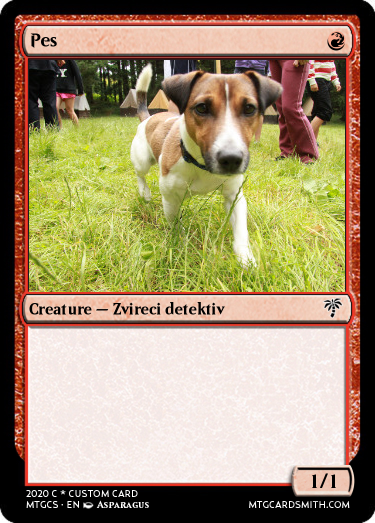
\includegraphics[scale=0.75]{cards/beginning/Pes.png}
        }
        \subfigure{
            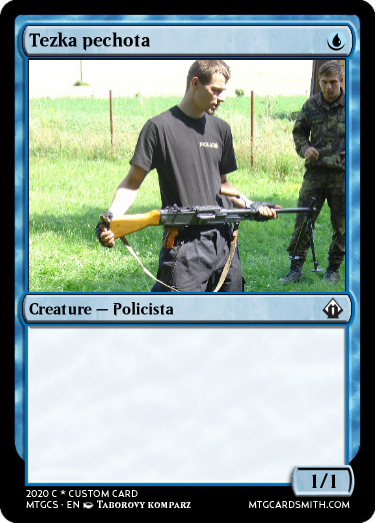
\includegraphics[scale=0.75]{cards/beginning/Tezka_pechota.png}
        }
        \subfigure{
            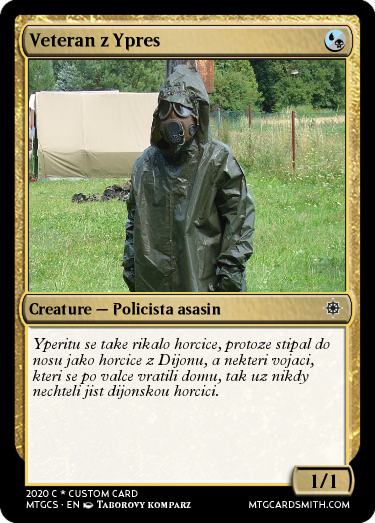
\includegraphics[scale=0.75]{cards/beginning/Veteran_z_Ypres.png}
        }\\
        
        \subfigure{
            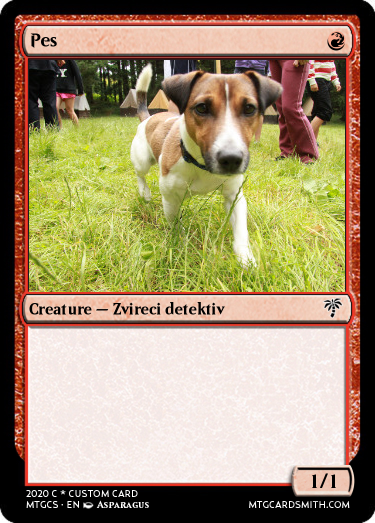
\includegraphics[scale=0.75]{cards/beginning/Pes.png}
        }
        \subfigure{
            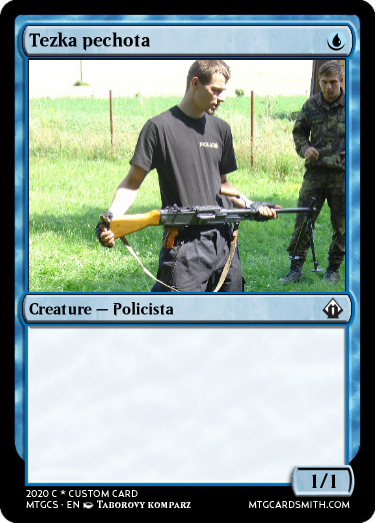
\includegraphics[scale=0.75]{cards/beginning/Tezka_pechota.png}
        }
        \subfigure{
            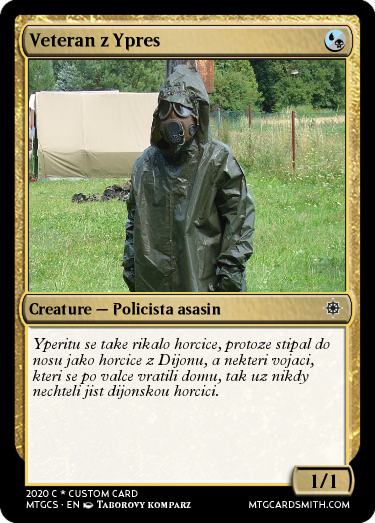
\includegraphics[scale=0.75]{cards/beginning/Veteran_z_Ypres.png}
        }
    \end{center}
\end{figure}

\advance \copy -1
\ifnum \copy>0
\repeat

% end of two copies

\documentclass{article}
\usepackage{subfigure}
\usepackage{lipsum}
\usepackage{graphicx}
\usepackage[utf8]{inputenc}
\usepackage{lscape}
\usepackage{pdfpages}
\usepackage{pgffor}

\usepackage[pass]{geometry}
\newgeometry{margin=0pt}
\usepackage[font=tiny,skip=0pt]{caption}

\extrafloats{1}

\begin{document}
\begin{landscape}

\newcommand*{\samples}
{
Hroznej_mastak,
Hroznej_mastak_1,
Hroznej_mastak_2,
Hroznej_mastak_3,
Hroznej_mastak_4,
Hroznej_mastak_5}

\newcommand{\type}{1000}

\newcounter{cards_line}
\newcounter{cards_page}
\newcounter{copy}

\setcounter{cards_line}{3}
\setcounter{cards_page}{6}
\setcounter{copy}{0}

\centering

\tiny{\type}

\loop
\foreach \x in \samples
{
	\includegraphics[scale=0.75]{cards/\type/\x.png}
	%
	\addtocounter{cards_line}{-1}
	\addtocounter{cards_page}{-1}
	\ifnum\value{cards_line} < 1
	
	\setcounter{cards_line}{3}
	\fi
	%
	\ifnum\value{cards_page} < 1
	\clearpage
	\tiny{\type}
	
	\setcounter{cards_page}{6}
	\fi
}
\addtocounter{copy}{1}
\ifnum\value{copy} < 3
\repeat

\end{landscape}
\end{document}

% now three copies

\newcount\copy
\copy=3
\loop

\documentclass{article}
\usepackage{subfigure}
\usepackage{lipsum}
\usepackage{graphicx}
\usepackage[utf8]{inputenc}
\usepackage{lscape}
\usepackage{pdfpages}
\usepackage{pgffor}

\usepackage[pass]{geometry}
\newgeometry{margin=0pt}
\usepackage[font=tiny,skip=0pt]{caption}

\extrafloats{1}

\begin{document}
\begin{landscape}

\newcommand*{\samples}
{
Cerny_bananovnik,
Cerny_bananovnik_1,
Cerny_bananovnik_2,
Cerny_bananovnik_3,
Cerny_bananovnik_4,
Cerveny_bananovnik,
Cerveny_bananovnik_1,
Cerveny_bananovnik_2,
Cerveny_bananovnik_3,
Cerveny_bananovnik_4,
Modry_bananovnik,
Modry_bananovnik_1,
Modry_bananovnik_2,
Modry_bananovnik_3,
Modry_bananovnik_4}

\newcommand{\type}{2000}

\newcounter{cards_line}
\newcounter{cards_page}
\newcounter{copy}

\setcounter{cards_line}{3}
\setcounter{cards_page}{6}
\setcounter{copy}{0}

\centering

\tiny{\type}

\loop
\foreach \x in \samples
{
	\includegraphics[scale=0.75]{cards/\type/\x.png}
	%
	\addtocounter{cards_line}{-1}
	\addtocounter{cards_page}{-1}
	\ifnum\value{cards_line} < 1
	
	\setcounter{cards_line}{3}
	\fi
	%
	\ifnum\value{cards_page} < 1
	\clearpage
	\tiny{\type}
	
	\setcounter{cards_page}{6}
	\fi
}
\addtocounter{copy}{1}
\ifnum\value{copy} < 3
\repeat

\end{landscape}
\end{document}

\documentclass{article}
\usepackage{subfigure}
\usepackage{lipsum}
\usepackage{graphicx}
\usepackage[utf8]{inputenc}
\usepackage{lscape}
\usepackage{pdfpages}
\usepackage{pgffor}

\usepackage[pass]{geometry}
\newgeometry{margin=0pt}
\usepackage[font=tiny,skip=0pt]{caption}

\extrafloats{1}

\begin{document}
\begin{landscape}

\newcommand*{\samples}
{
Bananova_laborator,
Bila_kralovna,
Cerna_sila,
Drin_japonsky,
Ekvadorsky_farmar,
Hodnej_polda,
Horka_davka,
Javsky_farmar,
Jedlik_Vetrniku,
Magicka_formule,
Mapa_bananoveho_souostrovi,
Modra_sila,
Nadrz_plna_leklych_bananu,
Praci_prasek_Arijec,
Ruda_sila,
Skliba,
Spekbrasnak,
Stado_falesnych_prasat,
Stylar,
Taboriste,
Thajsky_farmar,
Tradice_z_krabice,
Vetrna_elektrarna,
Vlajka_Francie}

\newcommand{\type}{4000}

\newcounter{cards_line}
\newcounter{cards_page}
\newcounter{copy}

\setcounter{cards_line}{3}
\setcounter{cards_page}{6}
\setcounter{copy}{0}

\centering

\tiny{\type}

\loop
\foreach \x in \samples
{
	\includegraphics[scale=0.75]{cards/\type/\x.png}
	%
	\addtocounter{cards_line}{-1}
	\addtocounter{cards_page}{-1}
	\ifnum\value{cards_line} < 1
	
	\setcounter{cards_line}{3}
	\fi
	%
	\ifnum\value{cards_page} < 1
	\clearpage
	\tiny{\type}
	
	\setcounter{cards_page}{6}
	\fi
}
\addtocounter{copy}{1}
\ifnum\value{copy} < 3
\repeat

\end{landscape}
\end{document}

\documentclass{article}
\usepackage{subfigure}
\usepackage{lipsum}
\usepackage{graphicx}
\usepackage[utf8]{inputenc}
\usepackage{lscape}
\usepackage{pdfpages}
\usepackage{pgffor}

\usepackage[pass]{geometry}
\newgeometry{margin=0pt}
\usepackage[font=tiny,skip=0pt]{caption}

\extrafloats{1}

\begin{document}
\begin{landscape}

\newcommand*{\samples}
{
Banadin,
Bedna_od_bananu,
Bedna_od_bananu_1,
Bily_vlk,
Cernobylsky_vagus,
Cernokneznik,
Doktor_Watson,
Dumpster_diver,
Fukusimska_posila,
Hra_nefer,
John_McLane,
Levak,
Mapa_bananove_plantaze,
Mynarova_zabijacka,
Nateraci,
Nocni_mury_pana_Hudopa,
Pneumatika,
Postak_snu,
Procitnuti,
Sennes,
SKWAT_tym,
Ukradena_vlajka,
Vagus_popelar,
Ve_znameni_lva}

\newcommand{\type}{6000}

\newcounter{cards_line}
\newcounter{cards_page}
\newcounter{copy}

\setcounter{cards_line}{3}
\setcounter{cards_page}{6}
\setcounter{copy}{0}

\centering

\tiny{\type}

\loop
\foreach \x in \samples
{
	\includegraphics[scale=0.75]{cards/\type/\x.png}
	%
	\addtocounter{cards_line}{-1}
	\addtocounter{cards_page}{-1}
	\ifnum\value{cards_line} < 1
	
	\setcounter{cards_line}{3}
	\fi
	%
	\ifnum\value{cards_page} < 1
	\clearpage
	\tiny{\type}
	
	\setcounter{cards_page}{6}
	\fi
}
\addtocounter{copy}{1}
\ifnum\value{copy} < 3
\repeat

\end{landscape}
\end{document}

\begin{figure}[ht!]
     \caption*{8000}
     \begin{center}
        \subfigure{
            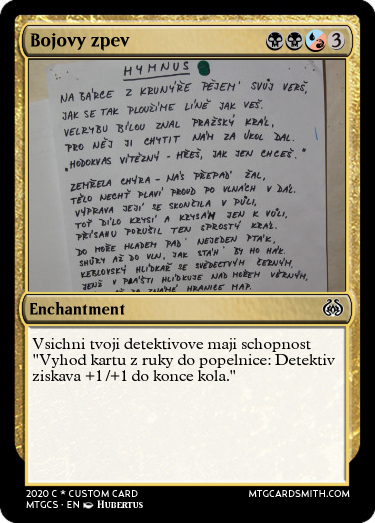
\includegraphics[scale=0.75]{cards/8000/Bojovy_zpev.png}
        }
        \subfigure{
            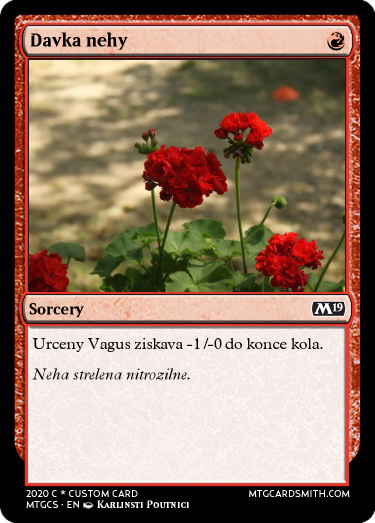
\includegraphics[scale=0.75]{cards/8000/Davka_nehy.png}
        }
        \subfigure{
            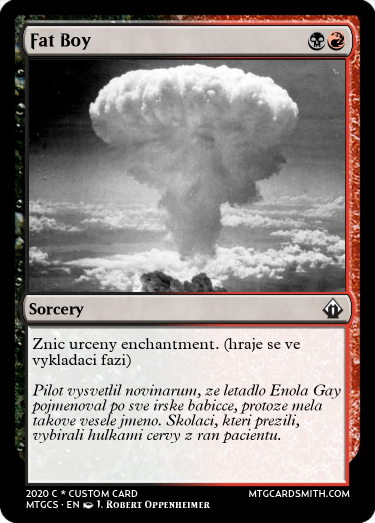
\includegraphics[scale=0.75]{cards/8000/Fat_Boy.png}
        }\\
        
        \subfigure{
            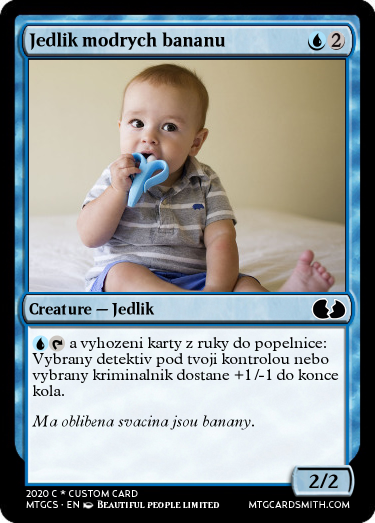
\includegraphics[scale=0.75]{cards/8000/Jedlik_modrych_bananu.png}
        }
        \subfigure{
            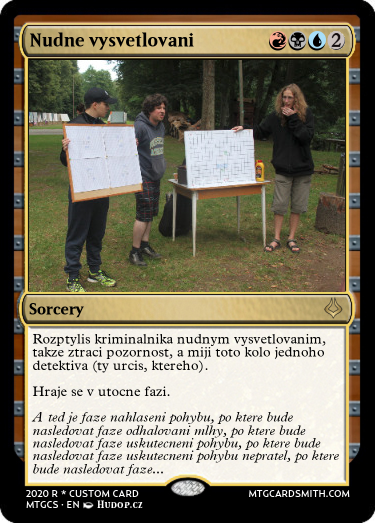
\includegraphics[scale=0.75]{cards/8000/Nudne_vysvetlovani.png}
        }
        \subfigure{
            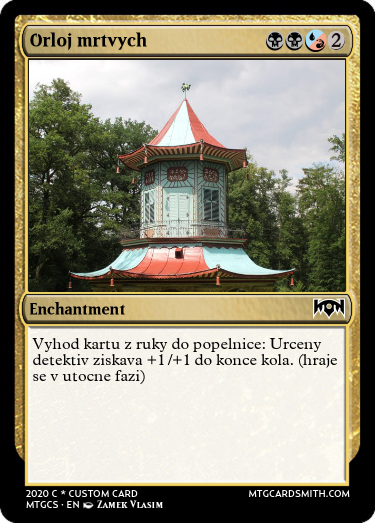
\includegraphics[scale=0.75]{cards/8000/Orloj_mrtvych.png}
        }
    \end{center}
\end{figure}

\begin{figure}[ht!]
     \caption*{8000}
     \begin{center}
        \subfigure{
            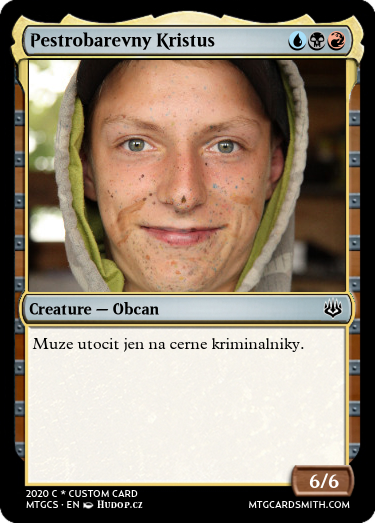
\includegraphics[scale=0.75]{cards/8000/Pestrobarevny_Kristus.png}
        }
        \subfigure{
            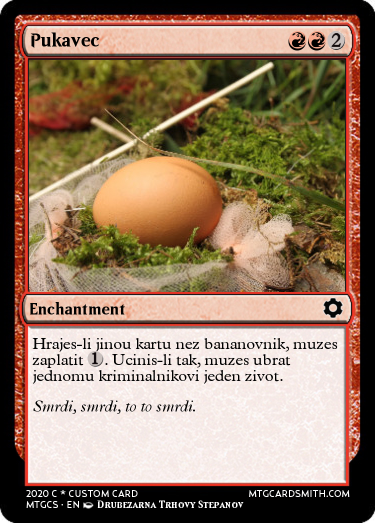
\includegraphics[scale=0.75]{cards/8000/Pukavec.png}
        }
        \subfigure{
            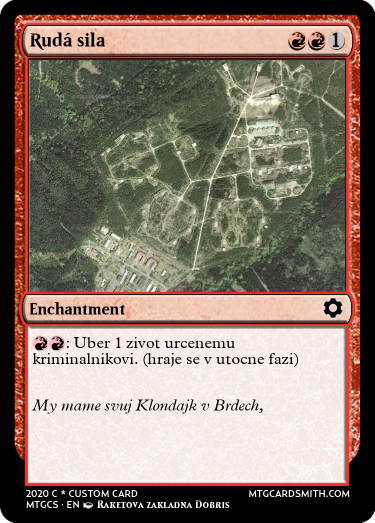
\includegraphics[scale=0.75]{cards/8000/Ruda_sila_Dobris.png}
        }\\
        
        \subfigure{
            
\includegraphics[scale=0.75]{cards/8000/Ruda_sila_z_Ostravy.png}
        }
        \subfigure{
            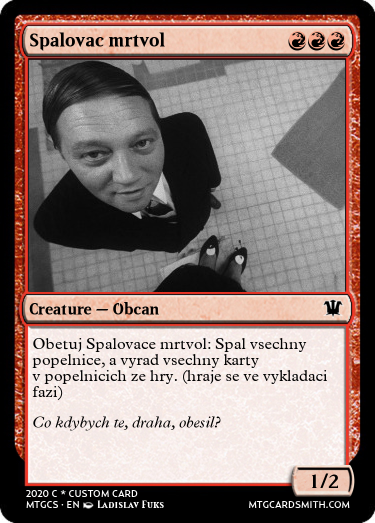
\includegraphics[scale=0.75]{cards/8000/Spalovac_mrtvol.png}
        }
        \subfigure{
            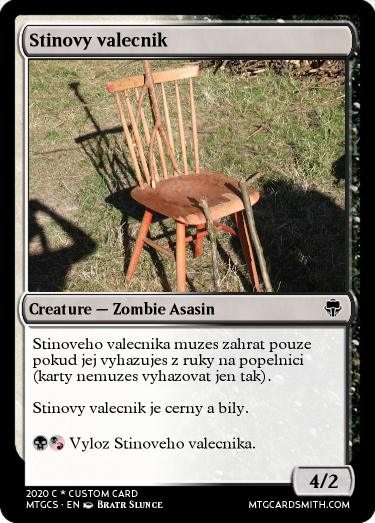
\includegraphics[scale=0.75]{cards/8000/Stinovy_valecnik.png}
        }
    \end{center}
\end{figure}

\begin{figure}[ht!]
     \caption*{8000}
     \begin{center}
        \subfigure{
            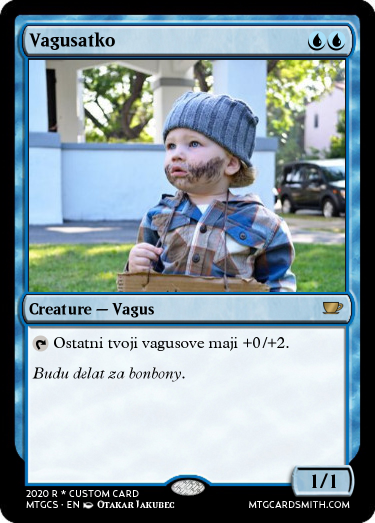
\includegraphics[scale=0.75]{cards/8000/Vagusatko.png}
        }
        \subfigure{
            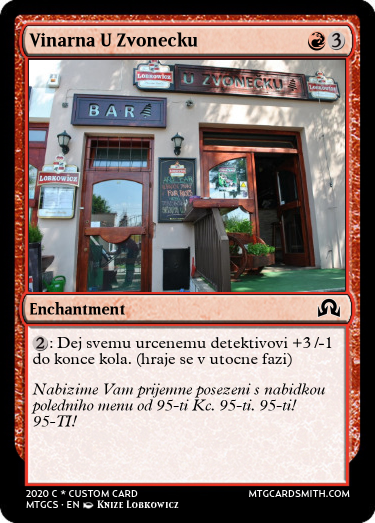
\includegraphics[scale=0.75]{cards/8000/Vinarna_U_Zvonecku.png}
        }
        \subfigure{
            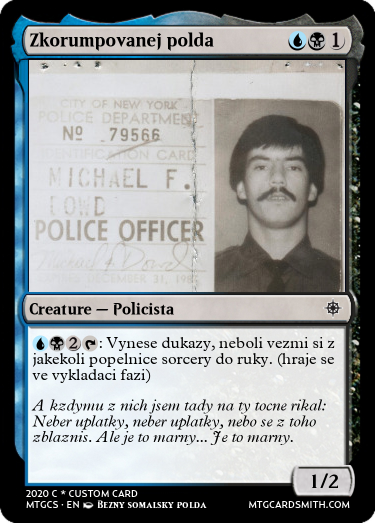
\includegraphics[scale=0.75]{cards/8000/Zkorumpovanej_polda.png}
        }\\
        
        \subfigure{
            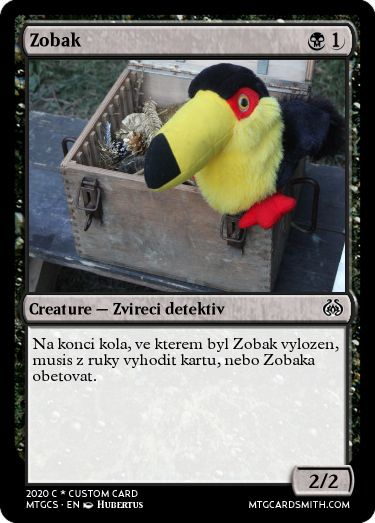
\includegraphics[scale=0.75]{cards/8000/Zobak.png}
        }
        \subfigure{
            
\includegraphics[scale=0.75]{cards/8000/Zuzivec.png}
        }
        \iffalse
        \subfigure{
            
\includegraphics[scale=0.75]{cards/8000/Zuzivec.png}
        }
        \fi
    \end{center}
\end{figure}

\begin{figure}[ht!]
     \caption*{10000}
     \begin{center}
        \subfigure{
            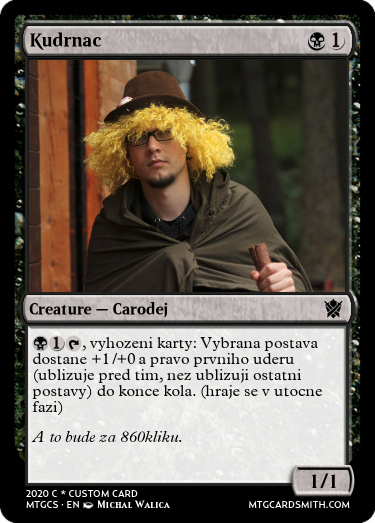
\includegraphics[scale=0.75]{cards/10000/Kudrnac.png}
        }
        \subfigure{
            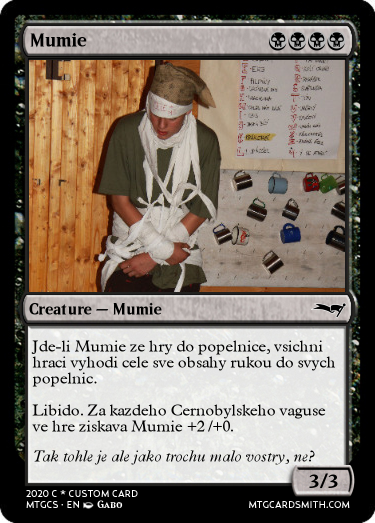
\includegraphics[scale=0.75]{cards/10000/Mumie.png}
        }
        \subfigure{
            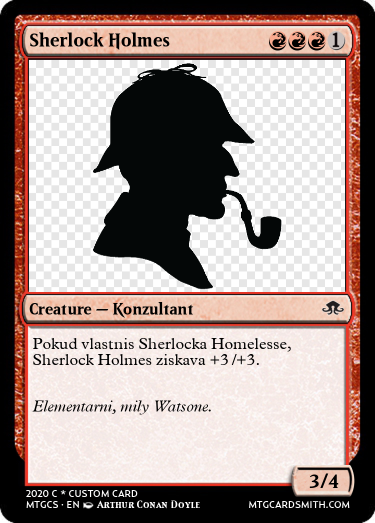
\includegraphics[scale=0.75]{cards/10000/Sherlock_Holmess.png}
        }\\
        
        \subfigure{
            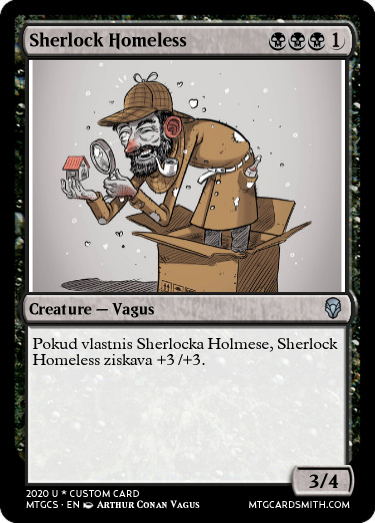
\includegraphics[scale=0.75]{cards/10000/Sherlock_Homeless.png}
        }
        \subfigure{
            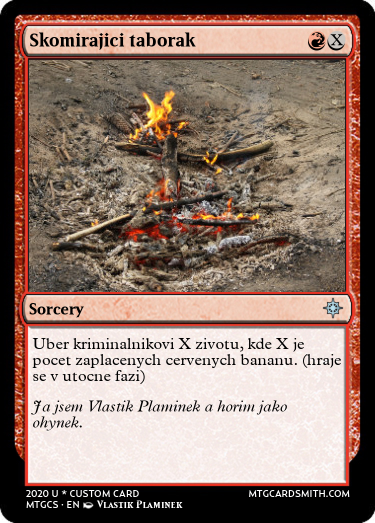
\includegraphics[scale=0.75]{cards/10000/Skomirajici_taborak.png}
        }
        \iffalse
        \subfigure{
            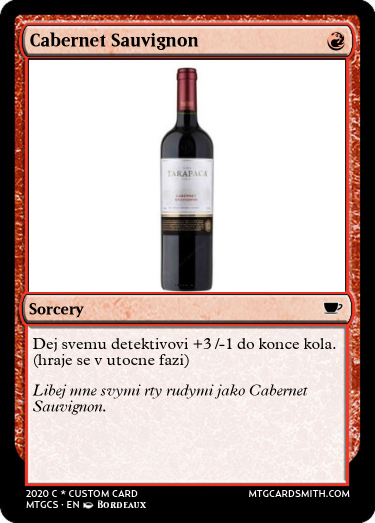
\includegraphics[scale=0.75]{cards/10000/Cabernet_Sauvignon.png}
        }
        \fi
    \end{center}
\end{figure}

\documentclass{article}
\usepackage{subfigure}
\usepackage{lipsum}
\usepackage{graphicx}
\usepackage[utf8]{inputenc}
\usepackage{lscape}
\usepackage{pdfpages}
\usepackage{pgffor}

\usepackage[pass]{geometry}
\newgeometry{margin=0pt}
\usepackage[font=tiny,skip=0pt]{caption}

\extrafloats{1}

\begin{document}
\begin{landscape}

\newcommand*{\samples}
{
AllChimpsAreBurnt,
AllColoursAreBlack,
AllCopsAreBeautiful,
Cabernet_Sauvignon,
Chch,
Jatka,
Odstrelovac,
Policajtuv_sen,
Pupa,
Snovy_archivar,
Vystoupeni_Ondreje_Hejmy}

\newcommand{\type}{12000}

\newcounter{cards_line}
\newcounter{cards_page}
\newcounter{copy}

\setcounter{cards_line}{3}
\setcounter{cards_page}{6}
\setcounter{copy}{0}

\centering

\tiny{\type}

\loop
\foreach \x in \samples
{
	\includegraphics[scale=0.75]{cards/\type/\x.png}
	%
	\addtocounter{cards_line}{-1}
	\addtocounter{cards_page}{-1}
	\ifnum\value{cards_line} < 1
	
	\setcounter{cards_line}{3}
	\fi
	%
	\ifnum\value{cards_page} < 1
	\clearpage
	\tiny{\type}
	
	\setcounter{cards_page}{6}
	\fi
}
\addtocounter{copy}{1}
\ifnum\value{copy} < 3
\repeat

\end{landscape}
\end{document}

\begin{figure}[ht!]
     \caption*{18000}
     \begin{center}
        \subfigure{
            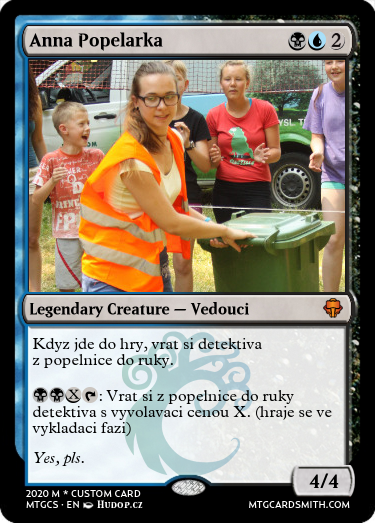
\includegraphics[scale=0.75]{cards/18000/Anna_Popelarka.png}
        }
        \subfigure{
            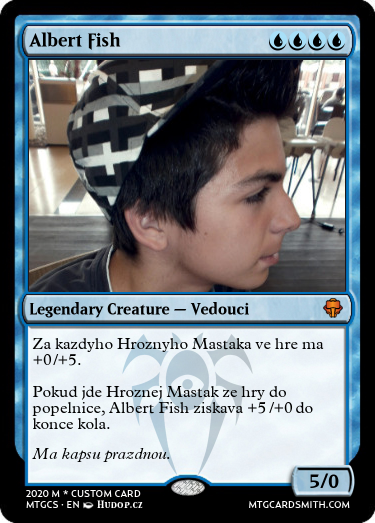
\includegraphics[scale=0.75]{cards/18000/Albert_Fish.png}
        }
        \subfigure{
            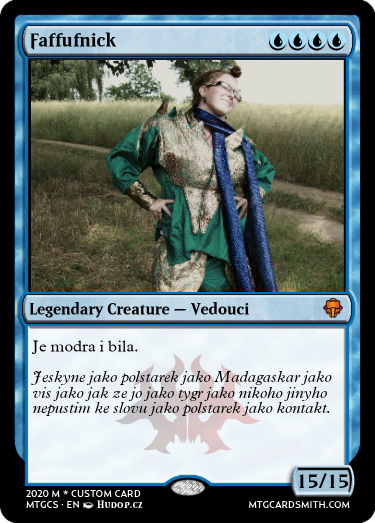
\includegraphics[scale=0.75]{cards/18000/Faffufnick.png}
        }\\
        \subfigure{
            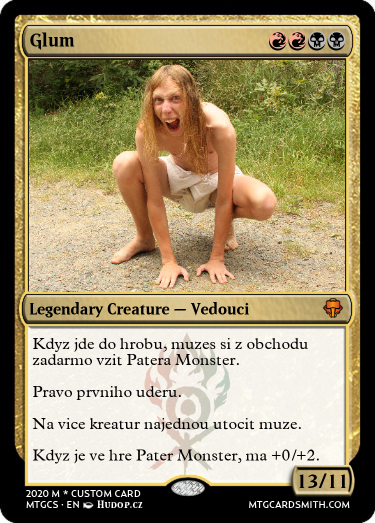
\includegraphics[scale=0.75]{cards/18000/Glum.png}
        }
        \subfigure{
            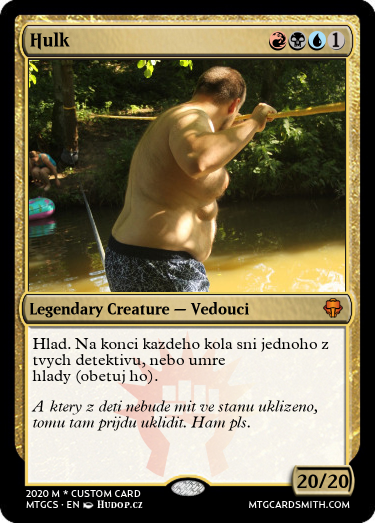
\includegraphics[scale=0.75]{cards/18000/Hulk.png}
        }
        \subfigure{
            \includegraphics[scale=0.75]{cards/18000/Jeji_Pastorkyna.png}
        }
    \end{center}
\end{figure}

\begin{figure}[ht!]
     \caption*{18000}
     \begin{center}
        \subfigure{
            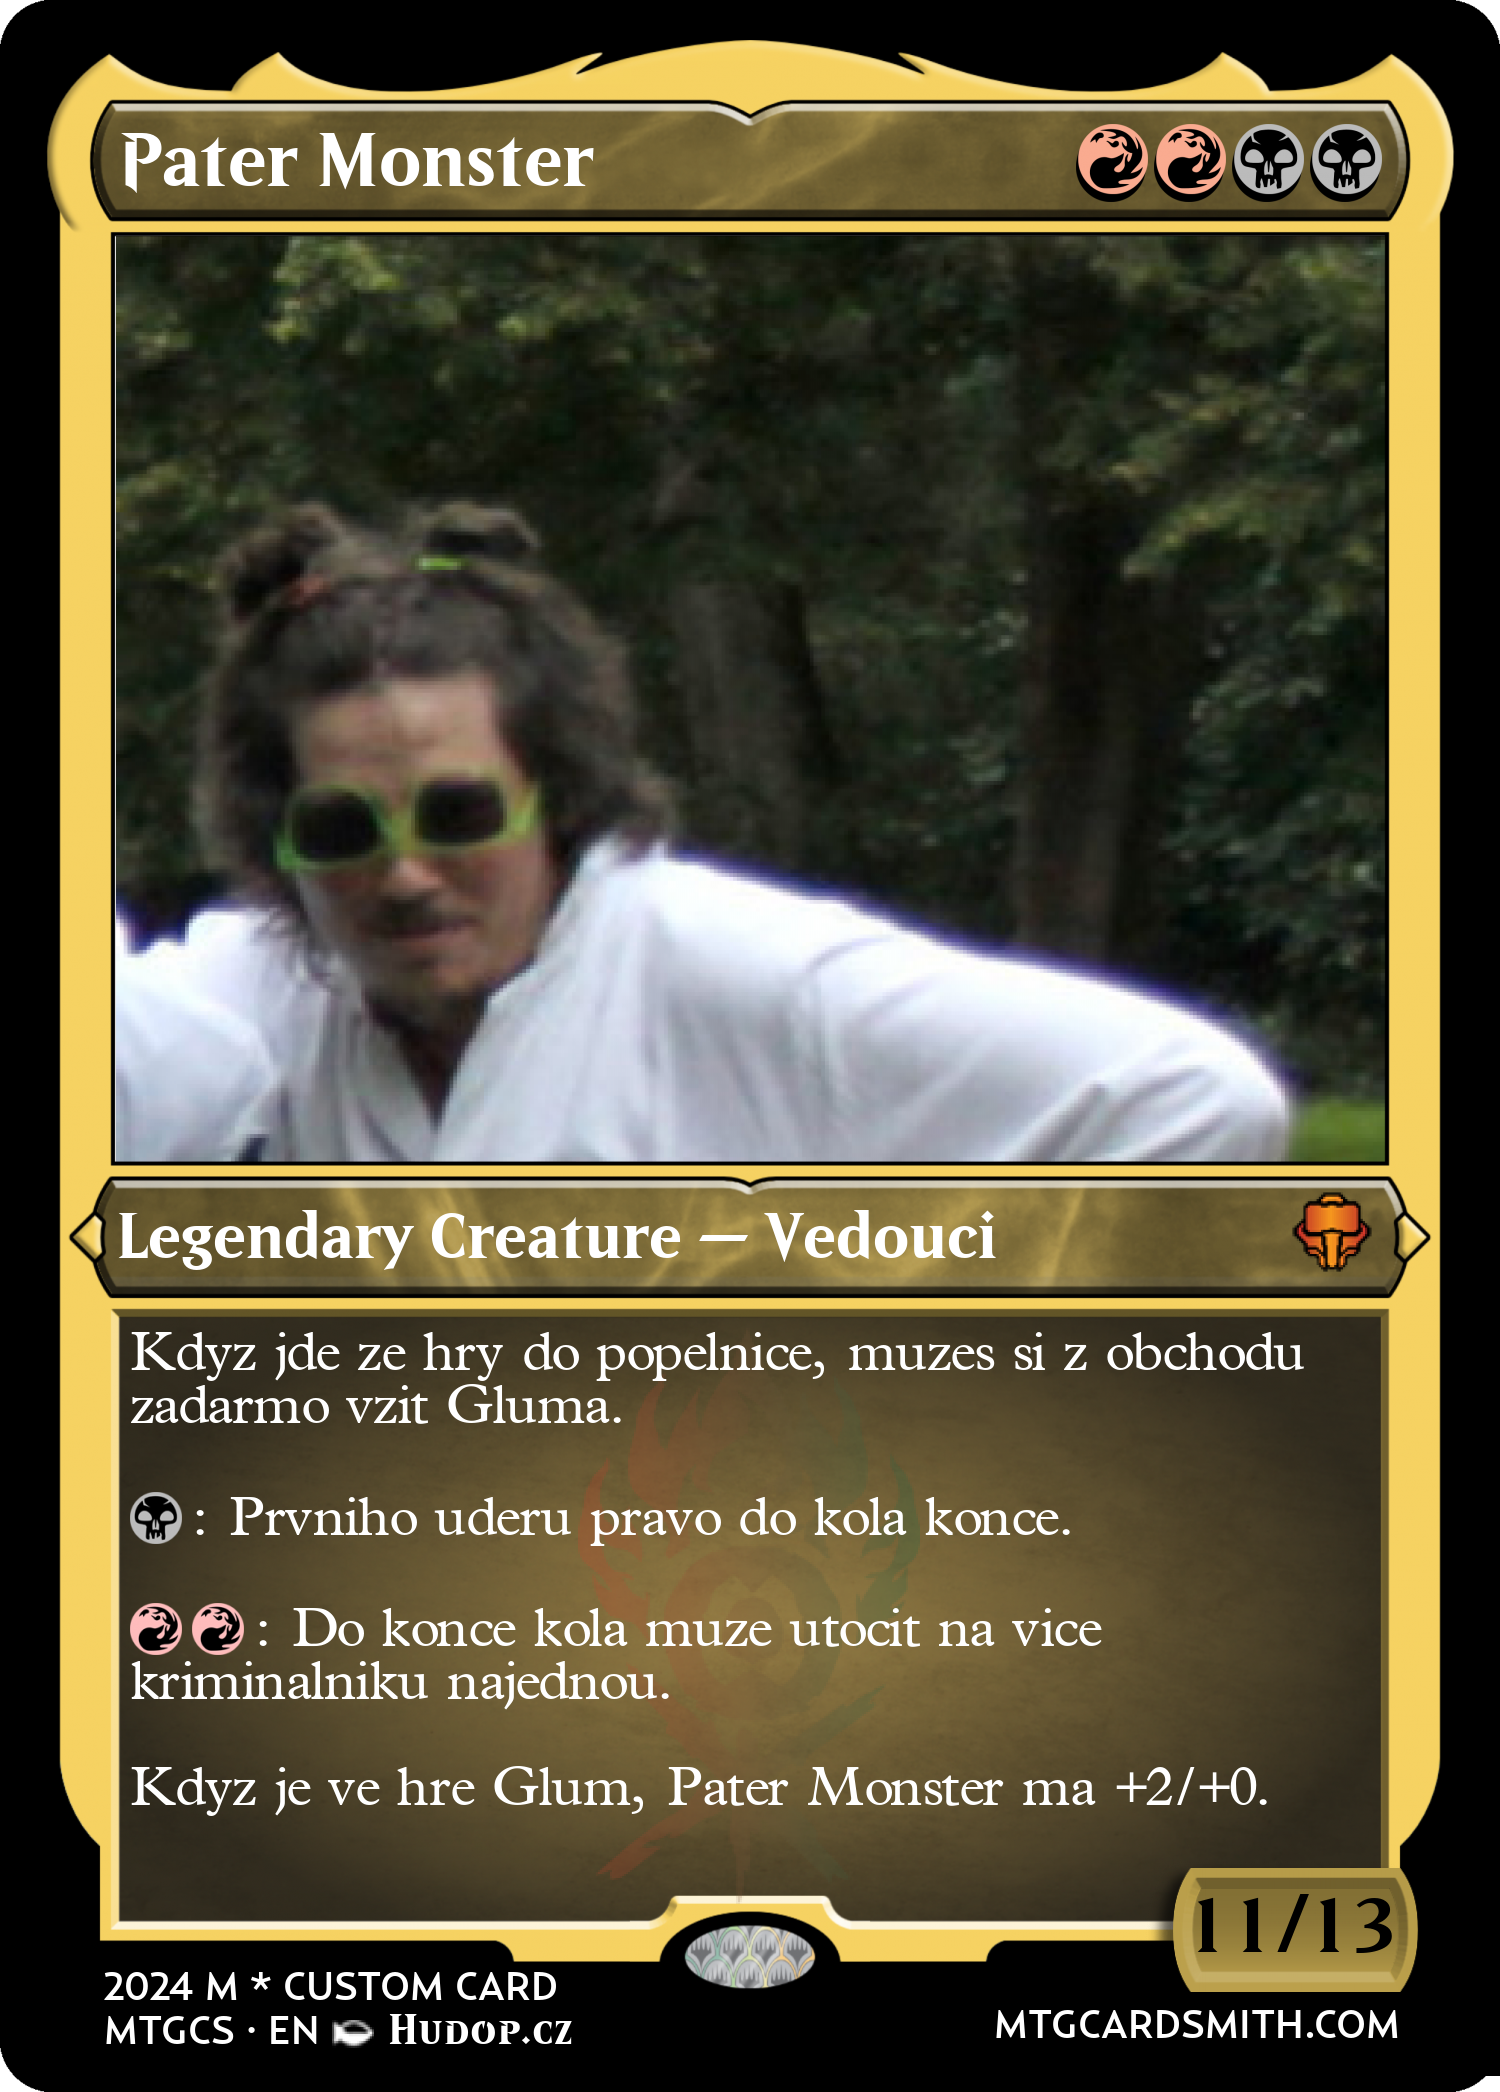
\includegraphics[scale=0.75]{cards/18000/Pater_Monster.png}
        }
        \subfigure{
            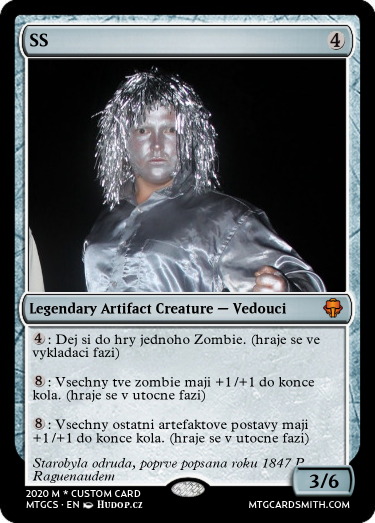
\includegraphics[scale=0.75]{cards/18000/SS.png}
        }
        \subfigure{
            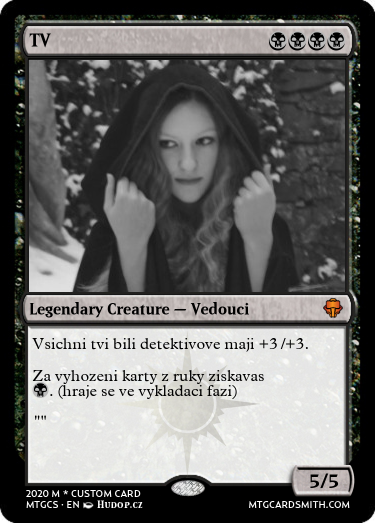
\includegraphics[scale=0.75]{cards/18000/TV.png}
        }\\
        
        \subfigure{
            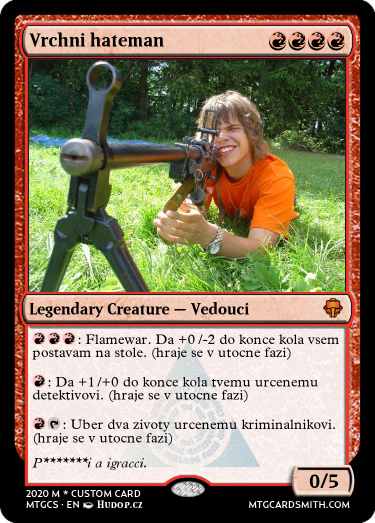
\includegraphics[scale=0.75]{cards/18000/Vrchni_hateman.png}
        }
        \iffalse
        \subfigure{
            \includegraphics[scale=0.75]{}
        }
        \subfigure{
            \includegraphics[scale=0.75]{}
        }
        \fi
    \end{center}
\end{figure}


\begin{figure}[ht!]
     \caption*{criminals}
     \begin{center}
        \subfigure{
            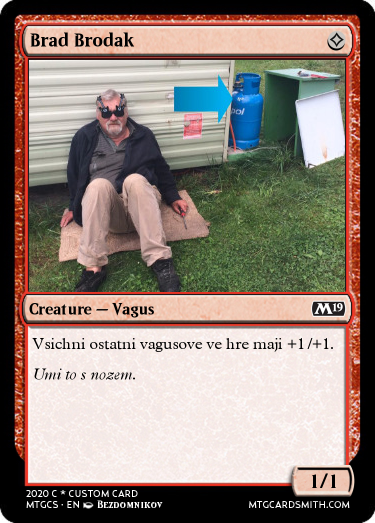
\includegraphics[scale=0.75]{cards/criminals/Brad_Brodak.png}
        }
        \subfigure{
            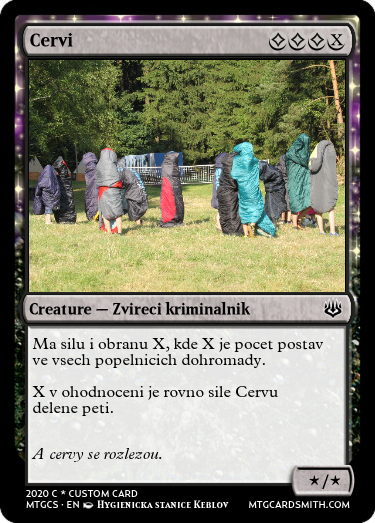
\includegraphics[scale=0.75]{cards/criminals/Cervi.png}
        }
        \subfigure{
            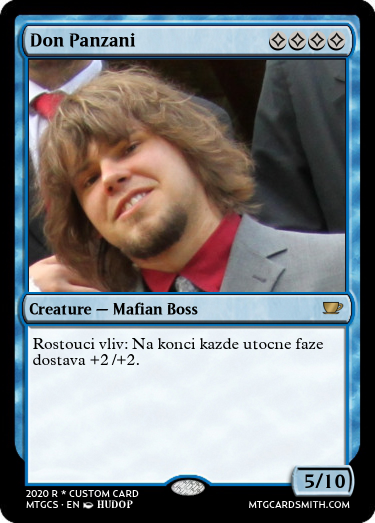
\includegraphics[scale=0.75]{cards/criminals/Don_Panzani.png}
        }\\
        
        \subfigure{
            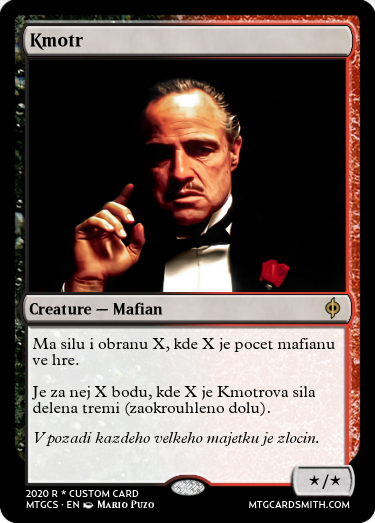
\includegraphics[scale=0.75]{cards/criminals/Kmotr.png}
        }
        \subfigure{
            
\includegraphics[scale=0.75]{cards/criminals/Kromerizske_trvanlive_salamy.png}
        }
        \subfigure{
            \includegraphics[scale=0.75]{cards/criminals/Lobo.png}
        }
    \end{center}
\end{figure}

\begin{figure}[ht!]
     \caption*{criminals}
     \begin{center}
        \subfigure{
            \includegraphics[scale=0.75]{cards/criminals/Margherita_Mafian.png}
        }
        \subfigure{
            \includegraphics[scale=0.75]{cards/criminals/Najemny_vrah.png}
        }
        \subfigure{
            \includegraphics[scale=0.75]{cards/criminals/Narkobaron.png}
        }\\
        
        \subfigure{
            \includegraphics[scale=0.75]{cards/criminals/Narkozombie.png}
        }
        \subfigure{
            \includegraphics[scale=0.75]{cards/criminals/Prisera_s_takovejma_tesakama.png}
        }
        \subfigure{
            \includegraphics[scale=0.75]{cards/criminals/Profesor_Moriarty.png}
        }
    \end{center}
\end{figure}

\begin{figure}[ht!]
     \caption*{criminals}
     \begin{center}
        \subfigure{
            \includegraphics[scale=0.75]{cards/criminals/PVS.png}
        }
        \subfigure{
            \includegraphics[scale=0.75]{cards/criminals/Sila_pozitivniho_vagusismu.png}
        }
        \subfigure{
            \includegraphics[scale=0.75]{cards/criminals/Skunk_pruhovany.png}
        }\\

        \subfigure{
            \includegraphics[scale=0.75]{cards/criminals/Skurut-hai.png}
        }
        \subfigure{
            \includegraphics[scale=0.75]{cards/criminals/Smazka.png}
        }
        \subfigure{
            \includegraphics[scale=0.75]{cards/criminals/Tlustoch_Johny.png}
        }
    \end{center}
\end{figure}

\begin{figure}[ht!]
     \caption*{criminals}
     \begin{center}
        \subfigure{
            \includegraphics[scale=0.75]{cards/criminals/Usaty_torpedo.png}
        }
        \subfigure{
            \includegraphics[scale=0.75]{cards/criminals/Vetrnik_zla.png}
        }
        \subfigure{
            \includegraphics[scale=0.75]{cards/criminals/Vyberci.png}
        }\\

        \subfigure{
            \includegraphics[scale=0.75]{cards/criminals/Zlej_polda.png}
        }
        \subfigure{
            \includegraphics[scale=0.75]{cards/criminals/Zlodejicek.png}
        }
        \iffalse
        \subfigure{
            \includegraphics[scale=0.75]{cards/criminals/.png}
        }
        \fi
    \end{center}
\end{figure}

\documentclass{article}
\usepackage{subfigure}
\usepackage{lipsum}
\usepackage{graphicx}
\usepackage[utf8]{inputenc}
\usepackage{lscape}
\usepackage{pdfpages}
\usepackage{pgffor}

\usepackage[pass]{geometry}
\newgeometry{margin=0pt}
\usepackage[font=tiny,skip=0pt]{caption}

\extrafloats{1}

\begin{document}
\begin{landscape}

\newcommand*{\samples}
{
Mafian,
Zombie,
Zvire_android}

\newcommand{\type}{tokens}

\newcounter{cards_line}
\newcounter{cards_page}
\newcounter{copy}

\setcounter{cards_line}{3}
\setcounter{cards_page}{6}
\setcounter{copy}{0}

\centering

\tiny{\type}

\loop
\foreach \x in \samples
{
	\includegraphics[scale=0.75]{cards/\type/\x.png}
	%
	\addtocounter{cards_line}{-1}
	\addtocounter{cards_page}{-1}
	\ifnum\value{cards_line} < 1
	
	\setcounter{cards_line}{3}
	\fi
	%
	\ifnum\value{cards_page} < 1
	\clearpage
	\tiny{\type}
	
	\setcounter{cards_page}{6}
	\fi
}
\addtocounter{copy}{1}
\ifnum\value{copy} < 10
\repeat

\end{landscape}
\end{document}

\advance \copy -1
\ifnum \copy>0
\repeat

% end of three copies

\end{landscape}
\end{document}